\documentclass{article}

\usepackage[french]{babel}
\usepackage[latin1]{inputenc}
\usepackage{mathtools}
\usepackage{graphicx}
\usepackage{float}

%%%%%%%%%%%%%%%% Lengths %%%%%%%%%%%%%%%%
\setlength{\textwidth}{15.5cm}
\setlength{\evensidemargin}{0.5cm}
\setlength{\oddsidemargin}{0.5cm}

%%%%%%%%%%%%%%%% Variables %%%%%%%%%%%%%%%%
\def\projet{5}
\def\titre{Interpolation and integration methods / Cubic splines and surface interpolation}
\def\groupe{2}
\def\equipe{1}
\def\responsible{cborc}
\def\secretary{htoussaint}
\def\others{rpetro, pmeyzen, amilliet}

\begin{document}

%%%%%%%%%%%%%%%% Header %%%%%%%%%%%%%%%%
\noindent\begin{minipage}{0.98\textwidth}
  \vskip 0mm
  \noindent
  { \begin{tabular}{p{7.5cm}}
      {\bfseries \sffamily
        Project n�\projet} \\ 
      {\itshape \titre}
    \end{tabular}}
  \hfill 
  \fbox{\begin{tabular}{l}
      {~\hfill \bfseries \sffamily Group n�\groupe\ - Team n�\equipe
        \hfill~} \\[2mm] 
      Responsible : \responsible \\
      Secretary : \secretary \\
      Programmers : \others
    \end{tabular}}
  \vskip 4mm ~

  ~~~\parbox{0.95\textwidth}{\small \textit{Summary~:} \sffamily The aim of this project was to implement a model representing the airflow around an airfoil. This was achieved through three steps. First the airfoil was refined into a sufficiently smooth curve, using cubic splines. Then the length of the curve had to be computed, using integration methods. Finally the airflow was modelled using a laminar model, and a map describing the pressure around the airfoil was computed.  }
  \vskip 1mm ~
\end{minipage}

%%%%%%%%%%%%%%%% Main part %%%%%%%%%%%%%%%%
\section*{Airfoil refinment}
This first part was aimed at refining the airfoil, consisting of a list of points, into a sufficently smooth curve. An airfoil is separated into two parts : the upper surface and the lower surface. First, an airfoil profile was arbitrarily selected from de UIUC database, and loaded as arrays of points, using a python function provided beforehand (load\_foil).\\

The $ex$ and $ey$ returned by this function are arrays containing only one integer each, namely the number of points in the upper surface and in the lower surface. A separation function had then to be implemented, in order to separate the different arrays, in order to obtain two distinct curves (one for the upper surface, another for the lower one).\\

Those curves had then to be sufficiently smoothed, in order to be properly used and easily integrated. This was achieved through cubic spline interpolation : a piecewise-polynomial curve joins the points of a given set, such that each polynomial equation between each point is at most of order 3, and such that the continuity, the first and the second derivative of the overall curve is preserved.\\

At first, a scipy function (interp1d) was used to compute the interpolation, in order to obtain a display of the wanted result (figure 1).\\

Then, a proper function had to be programmed, with the help of the functions and explanations given in the Numerical Recipes (spline and splint).

\begin{figure}[H]
  \begin{center}
  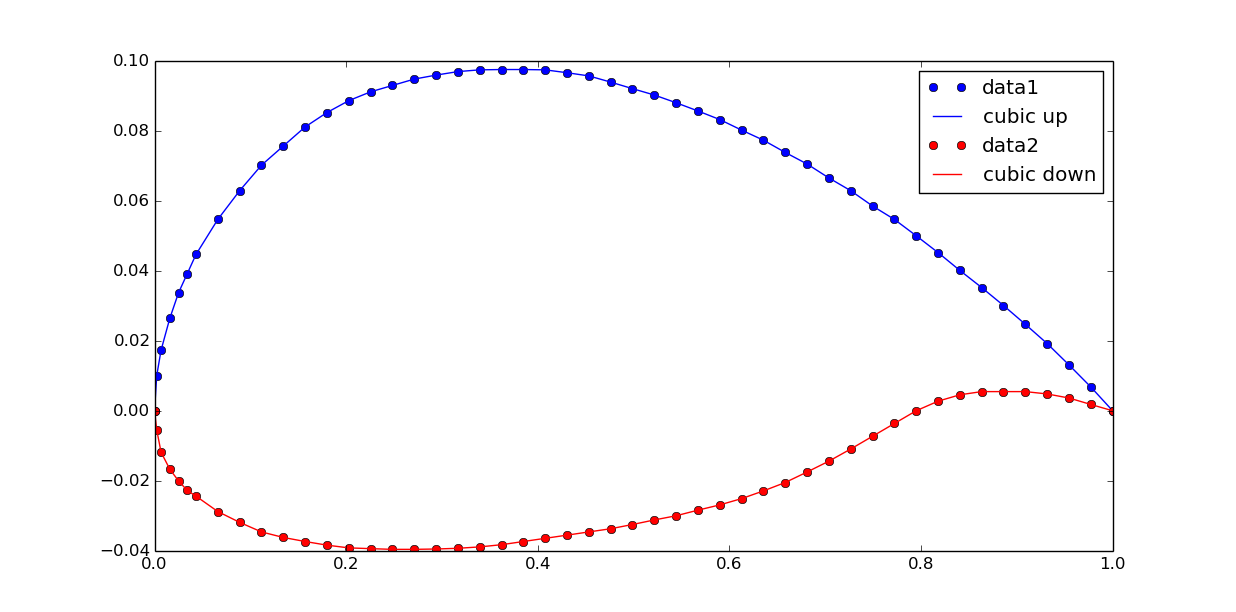
\includegraphics[scale=0.5]{figure_1.png}
  \end{center}
  \caption{Cubic spline interpolation of the upper (blue) and lower (red) surfaces}
\end{figure}





\section*{Computing the length of plane curves}

In this part, the aim was to compute the length of the curve, in order to obtain a pressure map in the last part of this project.
The splines are given as a function $x\rightarrow f(x)$ and the length of the curve can be calculated by the following integral :\\
\begin{equation*}
L([0;T]) = \displaystyle \int_0^T     \sqrt{1+f'(x)^2} ~dx
\end{equation*}

First of all, the derivative of the function f had to be computed (the code of this function is called ``derivation(x,esp)'' and is given in the source code). The derivative was calculated on several given points, therefore the first input ``y'' is a table. The second input ``eps'' is the step used to determine the derivative on each point.\\

Then, the length of the curve was computed by the function named ``length(y,a,b,n)'' where $y$ is a table of points, as previously described, a and b are the bounds of an interval, and n is the number of subsystems in this interval.\\

To compare the results and the speed of convergence, it was necessary to compute several integration methods.
In order to produce a generic tool, the integration method is a parameter of the function length, so the user can choose the method he wants to use to determine the length of the plane.\\

The integration method implemented in this project is called the rectangle method. This method consists in dividing the interval $[a,b]$ over which the function is to be integrated into $n$ equal subintervals of length $l$. The surface under the curve is then divided into rectangles of equal length l and whose heights are determined by the values of the function.\\
More specifically, the rectangles can be placed so that their left or right upper corner, or the middle of their top lign is exactly on the curve.\\
In the case of the upper right corner, the approximation of the integral is given by the following formula (using the parameters previously defined) :
\begin{equation*}
\displaystyle \int_a^b f(x)\,dx \approx l \sum_{k=1}^{n} f(a+kh)
\end{equation*}

\section*{Modelling the airflow}
After having drawn the shape of the airfoil and calculated the length of its curve, the goal of the last part was to model the behaviour of the airflow above and below the wing, following a laminar model.\\

The modelling of the airflow was computed following the instructions : \\
Every slice is given by the following function :
\begin{equation*}
y = f_{\lambda}(x) = (1-\lambda)f(x)+\lambda    \times 3h_{max} \qquad \forall \lambda \in [0;1]
\end{equation*}
Each slice matches to a certain value of $\lambda$.
In our example, $h_{max} \approx 0.10$ and $h_{min} \approx -0.04$, and 20 slices were drawn, as shown in figure 2.

\begin{figure}[H]
  \begin{center}
  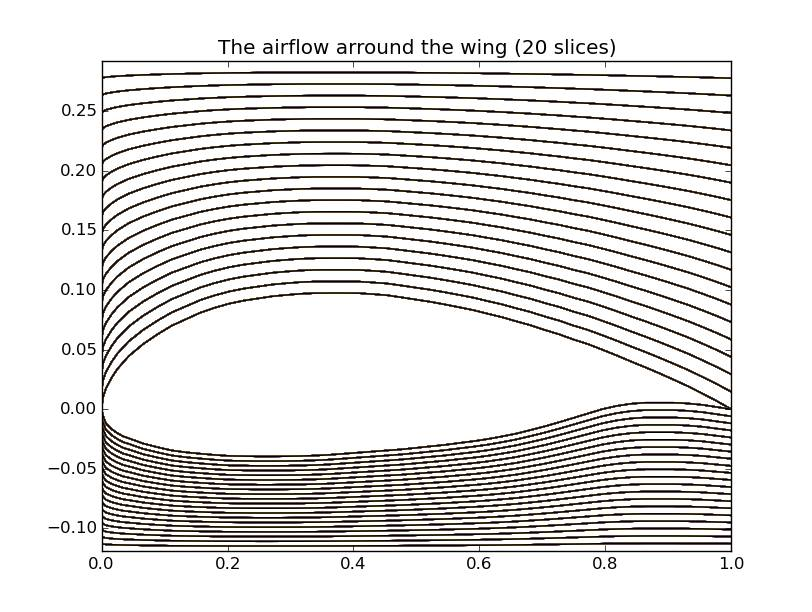
\includegraphics[scale=0.35]{figure_2.jpg}
  \end{center}
  \caption{Laminar flow above and below the airfoil}
\end{figure}

Finally, in order to draw the pressure map of the air above and below the wing, a matrix containing the values of the pressure at each point had to be computed, using the formula given in the instructions (the Bernoulli law). The pressure is indeed proportional to the speed squared. Moreover, on each slice of the laminar flow, the pressure is equal on every point of the slice. For example, on every point of the slice closest to the upper side of the airfoil, the pressure is equal and maximal.\\
This is where the length of the curve calculated in the previous section comes into use : the speed is calculated by computing the length of each slice, represented by the aforementioned $f_{\lambda}$ functions.\\
At the moment, the pressure map is not properly drawn in our program.
\end{document}
